%%%%%%%%%%%%%%%%%%%%%%%%%%%%%%%%%%%%%%%%%%%%%%%%%%%%%%%%%%%%%%%%%%%%%%%%%%%%%%%
%
% Tommy P. Keane
% Master of Science Thesis
% Department of Electrical and Microelectronic Engineering
%
% March 2011
%
%
%
% .tex and .sty modified from:
% http://www.ce.rit.edu/studentresources/gradresource/LaTexThesis.zip
%
%%%%%%%%%%%%%%%%%%%%%%%%%%%%%%%%%%%%%%%%%%%%%%%%%%%%%%%%%%%%%%%%%%%%%%%%%%%%%%%

%%%%%%%%%%%%%%%%%%%%%%%%%%%%%%%%%%%%%%%%%%%%%%%%%%%%%%%%%%%%%%%%%%%%%%%%%%%%%%%
%
% CHAPTER 5
%
% SECTION 3
%
%%%%%%%%%%%%%%%%%%%%%%%%%%%%%%%%%%%%%%%%%%%%%%%%%%%%%%%%%%%%%%%%%%%%%%%%%%%%%%%


%%%%%%%%%%%%%%%%%%%%%%%%%%%%%%%%%%%%%%%%%%%%%%%%%%%%%%%%%%%%%%%%%%%%%%%%%%%%%%%
% BEGIN DOCUMENT

TO BE WRITTEN

% ART GALLERY 001
\begin{figure}[!h]
\centering
\subfigure[]{ 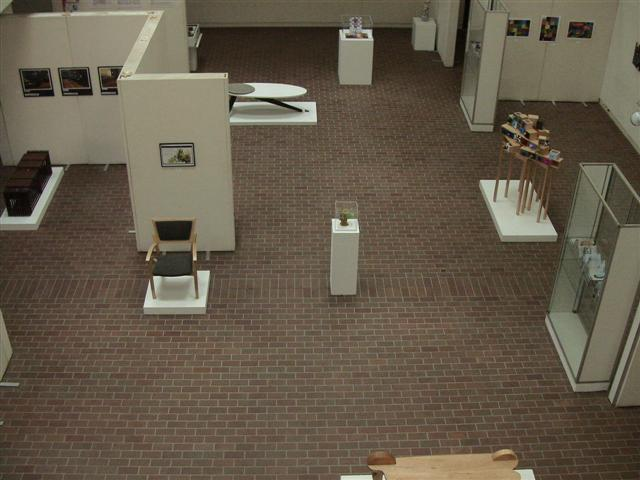
\includegraphics[width=.45\textwidth]{AGS1L001} \label{ArtGallery1L} }
\subfigure[]{ 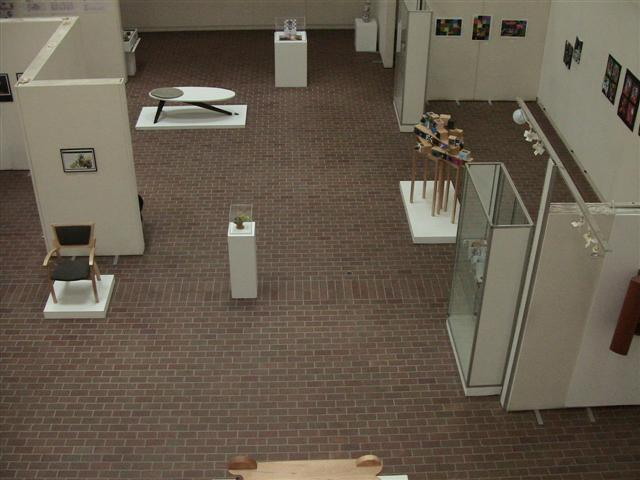
\includegraphics[width=.45\textwidth]{AGS1R001} \label{ArtGallery1R} }
\caption{Art Gallery Scene 01 (a) Left View, (b) Right View}
\label{ArtGallery1Images}
\end{figure}

\begin{figure}[!h]
\label{ArtGallery1Stitched}
\centering
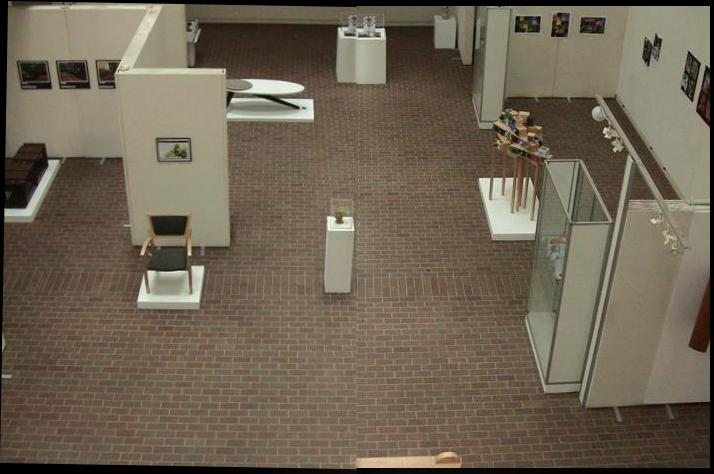
\includegraphics[width=1\textwidth]{AGS1SP001001}
\caption{Art Gallery 01 Views Blended}
\end{figure}




% ART GALLERY 002
\begin{figure}[!h]
\label{ArtGallery2Images}
\centering
\subfigure[]{ 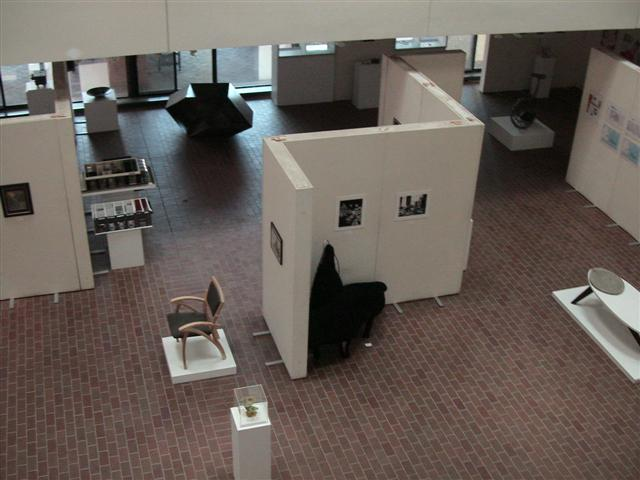
\includegraphics[width=.45\textwidth]{AGS2L001} \label{ArtGallery2L} }
\subfigure[]{ 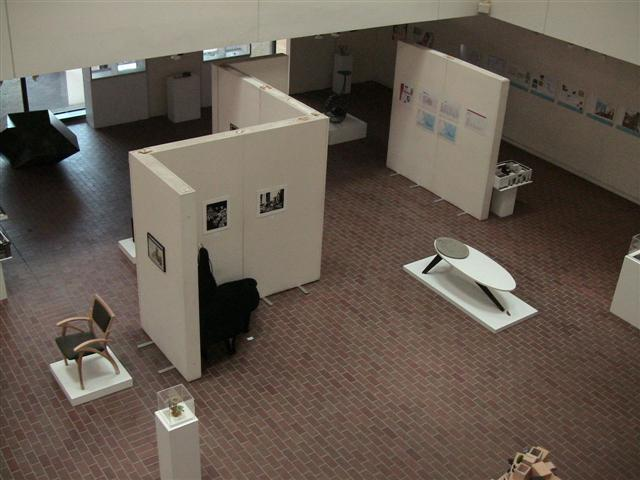
\includegraphics[width=.45\textwidth]{AGS2R001} \label{ArtGallery2R} }
\caption{Art Gallery Scene 02 (a) Left View, (b) Right View}
\end{figure}

\begin{figure}[!h]
\label{ArtGallery2Stitched}
\centering
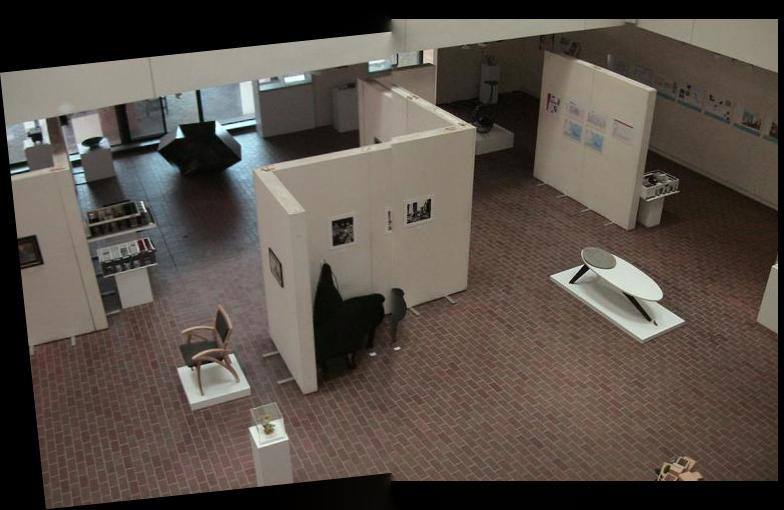
\includegraphics[width=1\textwidth]{AGS2SP001001}
\caption{Art Gallery 02 Views Blended}
\end{figure}



% LENEL 005
\begin{figure}[!h]
\label{Lenel5Images}
\centering
\subfigure[]{ 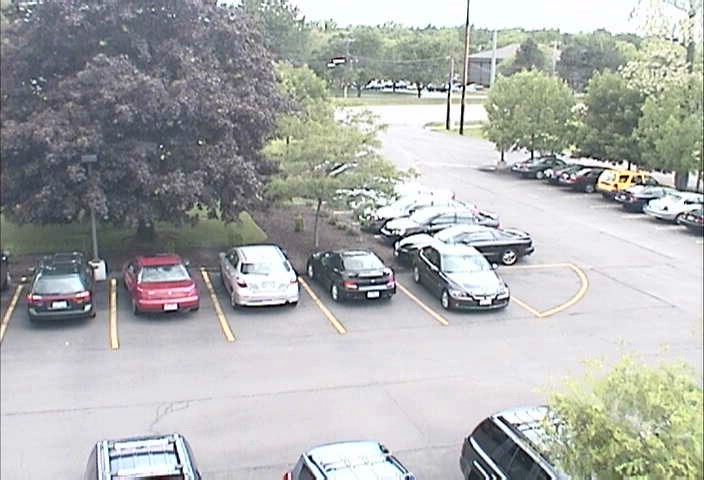
\includegraphics[width=.45\textwidth]{Lenel005L001} \label{Lenel5L} }
\subfigure[]{ 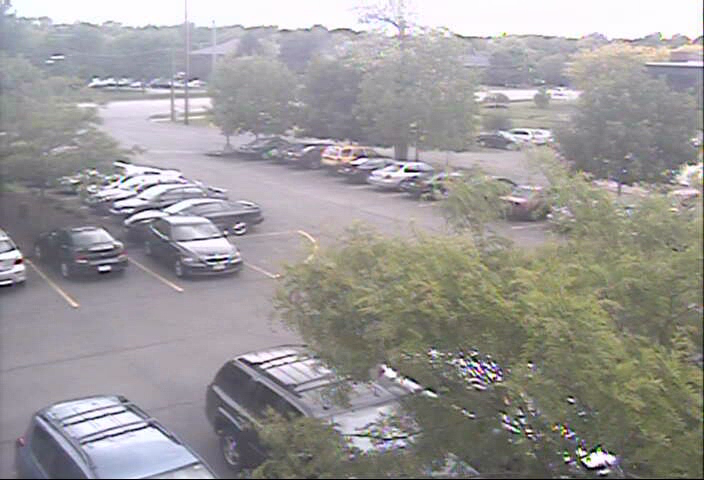
\includegraphics[width=.45\textwidth]{Lenel005R001} \label{Lenel5R} }
\caption{Lenel Front Lot Scene (a) Left View, (b) Right View}
\end{figure}

\begin{figure}[!h]
\label{Lenel5Stitched}
\centering
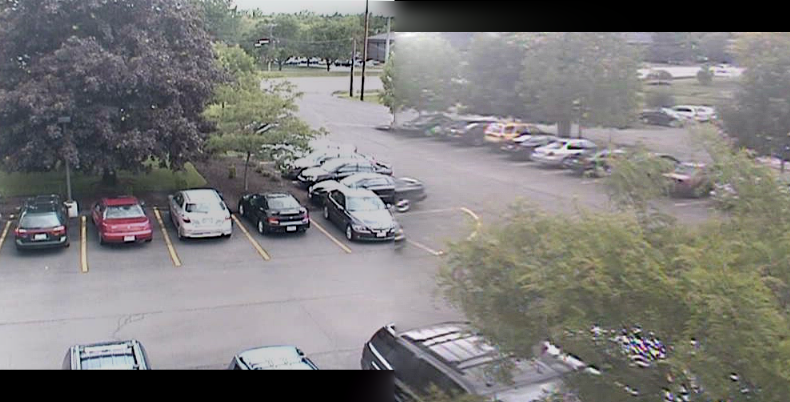
\includegraphics[width=1\textwidth]{Lenel005SP001001}
\caption{Lenel Front Lot Views Blended}
\end{figure}



% LENEL 010
\begin{figure}[!h]
\centering
\subfigure[]{ 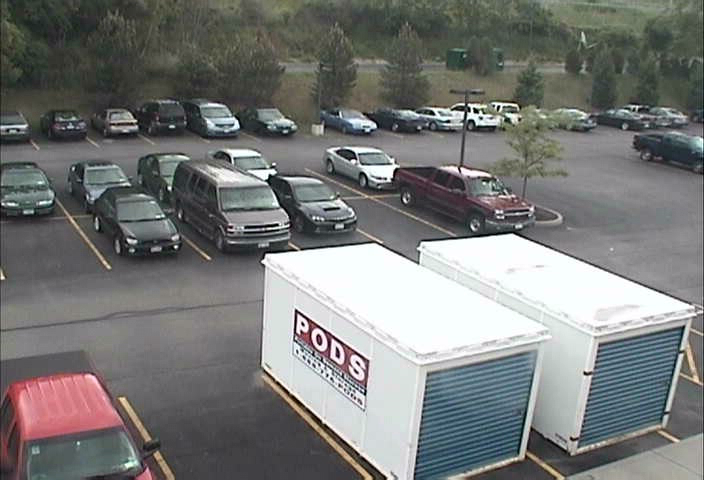
\includegraphics[width=.45\textwidth]{Lenel010L004} \label{Lenel10L} }
\subfigure[]{ 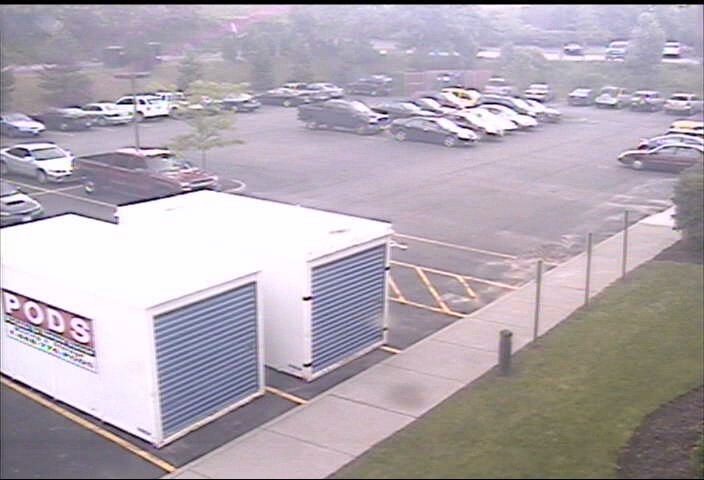
\includegraphics[width=.45\textwidth]{Lenel010R004} \label{Lenel10R} }
\caption{Lenel Back Lot Scene (a) Left View, (b) Right View}
\label{Lenel10Images}
\end{figure}

\begin{figure}[!h]
\centering
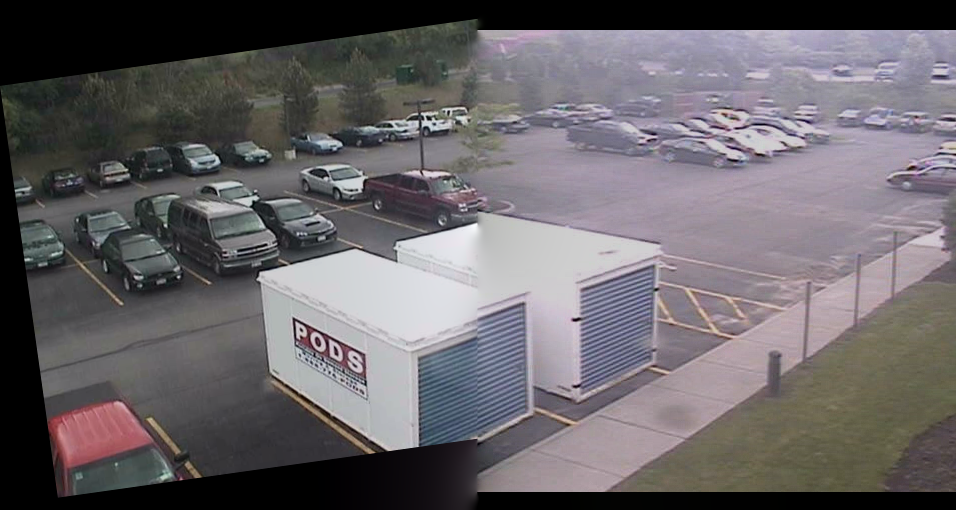
\includegraphics[width=1\textwidth]{Lenel010SP001}
\caption{Lenel Back Lot Views Blended}
\label{Lenel10Stitched}
\end{figure}


%%%%%%%%%%%%%%%%%%%%%%%%%%%%%%%%%%%%%%%%%%%%%%%%%%%%%%%%%%%%%%%%%%%%%%%%%%%%%%%
% END OF DOCUMENT

